\documentclass{IEEEtran}
\usepackage{cite}
\usepackage{amsmath,amssymb,amsfonts}
\usepackage{algorithm}
\usepackage{algorithmic}
\usepackage{graphicx}
\usepackage{textcomp}
\usepackage{subfigure}

\newcommand{\brho}{\boldsymbol{\rho}}
\newcommand{\brhop}{\boldsymbol{\rho^\prime}}
\newcommand{\Es}{\mathbf{E^S}}
\newcommand{\GS}{\mathbf{G^S}}
\newcommand{\X}{\boldsymbol{\chi}}
\newcommand{\E}{\mathbf{E}}
\newcommand{\Xo}{\boldsymbol{\bar{\chi}_o}}
\newcommand{\Xr}{\boldsymbol{\bar{\chi}_r}}

\begin{document}

    \title{To Be Decided}
    \author{Andr\'e Costa Batista, Ricardo Adriano, and Lucas S. Batista
        \thanks{This work has been supported by the Brazilian agencies Coordination for the Improvement of Higher Education Personnel - Brazil (CAPES) through the Academic Excellence Program (PROEX) under Grant 88887.815891/2023-00, FAPEMIG (Research Support Foundation of the State of Minas Gerais), and CNPq (The National Council for Scientific and Technological Development).}
        \thanks{A. C. Batista, R. Adriano, and L. S. Batista are with the Department of Electrical Engineering, Universidade Federal de Minas Gerais, Belo Horizonte, MG 31270-901, Brazil (e-mail: andre-costa@ufmg.br; rluiz@ufmg.br; lusoba@ufmg.br). A. C. Batista and L. S. Batista are also with Operations Research and Complex Systems Laboratory (ORCS Lab), Belo Horizonte, MG, Brazil.}}
   
    \maketitle
    
    \begin{abstract}
        To be written.
    \end{abstract}
    
    \begin{IEEEkeywords}
        Keyword 1, keyword 2, keyword 3. Remember: alphabetical order.
    \end{IEEEkeywords}
    
    \section{Introduction}\label{sec:introduction}
    
        \IEEEPARstart{H}{ere} we go.
        
        % O que é Microwave Imaging.
        
        % O papel dos algoritmos de inversão dentro de MWI para resolver o problema de espalhamento eletromagnético e quais desafios (ill-posedness etc). Destacar também a formulação 2D.
        
        % Quais classes de algoritmos e o que existe de mais novo.
        
        % Quais formas de avaliar soluções e quais ferramentas já existem (incluir aquele trabalho do Kurrant que é software para câncer de mama).
        
        % Descrever a lacuna para proposição de outros indicadores, tais como de posição e forma. Introduzir a minha proposta destacando vantagens, desvantagens e originalidade.
        
        % Organização do texto
        
	\section{Problem Statement}\label{sec:problemstatement}
		
		Let $D \in \mathbb{R}^2$ denote the Domain of Interest (DOI) embedded within a homogeneous, isotropic, nonmagnetic ($\mu = \mu_0 = 4\pi \times 10^{-7}$ H/m), and lossless ($\sigma = \sigma_0 = 0$ S/m) background medium with permittivity $\epsilon_b = \epsilon_{rb}\epsilon_0$, where $\epsilon_0 \approx 8.85 \times 10^{-12}$ F/m. We consider a 2D Transverse Magnetic (TMz) polarization where the DOI is illuminated by incident plane waves and assume the time convention $e^{j\omega t}$. All scatterers are located within the DOI, and the scattered field $E^s_z$ at point $\brho \in S$ outside $D$ is evaluated according to the following integral equation \cite{harrington2001time}:
		\begin{equation}
			E^s_z (\brho) = -\frac{k_b^2}{4} \int_D H_0^{(2)}(k_b|\brho-\brhop|)\chi(\brhop)E_z(\brhop) dS^\prime
		\end{equation}
		
		\noindent where $k_b = \omega\sqrt{\epsilon_b\mu_0} = 2\pi/\lambda_b$ is the background wave number, $\lambda_b$ is the wavelength of the incident wave, $H_0^{(2)}$ is the zero-order Hankel function of the second kind, $E_z$ is the total electric field in the DOI, and $\chi$ is the contrast function given by
		\begin{equation}
			\chi(\brho) = \frac{\epsilon_r(\brho)}{\epsilon_{rb}} - 1 - j\frac{\sigma(\brho)}{\omega\epsilon_b},
		\end{equation}
		
		\noindent which maps the relative permittivity $\epsilon_r(\brho)$ and conductivity $\sigma(\brho)$ distributions within $D$. It should be noted that the term $(-jk_b^2/4) H_0^{(2)}(k_b|\brho-\brhop|)$ corresponds to the Green's function in free space.
		
		In electromagnetic inverse scattering problems, we aim to recover the contrast function $\chi$ using a set of $N_M$ measurements of the scattered field collected for each of the $N_S$ sources. Additionally, $E_z$ is also unknown in $D$ and must be solved. For our formulation, the $N_S$ sources correspond to $N_S$ incidence angles of the plane wave, and the $N_M$ measurements are taken at $N_M$ points in $S$, arranged in a circular, equidistant array situated far from the center of the DOI by a radius $R_O$. By discretizing the DOI into $N_X \times N_Y = N$ pixels, the inverse problem is solved numerically according to the following equation:
		\begin{equation}
			E^s_{ms} = - \sum\limits_{n=1}^{N} G^S_{mn}\chi_{n}E_{ns} \label{eq:numerical}
		\end{equation}
		
		\noindent where $G^S$ is given according to the Richmond discretization \cite{richmond1965scattering, pastorino2010ch3}. Equation \eqref{eq:numerical} can also be expressed in matrix form:
		\begin{equation}
			\Es = \GS\X\E
		\end{equation}
		
		\noindent where $\Es$ is the $N_M \times N_S$ scattered field matrix, $\GS$ is the $N_M \times N$ Green's function matrix, $\X$ is the $N \times N$ contrast diagonal matrix, and $\E$ is the $N \times N_S$ total electric field matrix.
		
		It is important to highlight that, although assumptions are made regarding the scattered field domain and the incident field, the proposed indicators do not depend on these assumptions. They can be applied in any scenario where these entities are defined, and the assumptions in this paper serve only to clearly establish the context in which the indicators are tested.
	
	\section{Indicators}\label{sec:indicators}

		
		Once the result of the contrast function reconstruction is obtained by a given algorithm, the error in recovering the shape and location of the objects can be measured by comparing it with the original images. This means that the application of these metrics is relevant in studies where the exact response is known. Although in many real-world scenarios the imaged scatterer is unknown, applying these metrics to known cases can be valuable for comparing the performance of different algorithms and for estimating a confidence interval for the average performance of an algorithm in a given configuration. Therefore, these metrics are relevant tools that can contribute to the investigation and evaluation of algorithms for the problem.
		
		For the two indicators that will be explained below, the image of the original contrast function of the problem and the image reconstructed by any algorithm will be denoted by the matrices $\Xo$ and $\Xr$, both of size $N_X \times N_Y$. In other words, the elements of these matrices represent the pixels of the images.

		% Pressupostos:
		% 1. Função contraste (mapa) não seja uma função diferenciável (superfície).
		% 2. O algoritmo de reconstrução consegue discenir razoavelmente as bordas.
		% 3. No caso de múltiplos espalhadores com diferentes níveis de contraste, os menores níveis de constraste não estão abaixo da metade da diferença entre objeto de maior contraste e o fundo (**não ter contraste menor que zero**).
		% 4. Objetos de constraste diferentes não estejam sobrepostos (senão serão considerados como um objeto só).
	
		\subsection{Shape Error}\label{sec:indicators:shapeerror}
		
			% A função contraste tem valores complexos quando o meio ou os espalhadores possuem perdas. Portanto, o primeiro passo é tratar da possibilidade dos elementos das matrizes $\Xo$ e $\Xr$ terem partes reais e imaginárias. A abordagem mais simples é tomarmos o módulo das variáveis complexas como o valor de cada pixel. Esta escolha não elimina a possibilidade de que objetos com contrastes diferentes tenham o mesmo módulo. No entanto, nos casos onde somente existem materiais sem-perdas, esta abordagem não é problema porque o contraste é puramente real. Ao mesmo tempo, como o objetivo é verificar a forma dos espalhadores, o mais importante é fazer a separação entre meio-de-fundo e espalhador, sendo que o meio-de-fundo tem contraste zero. Portanto, esta escolha para simplificar a metodologia para mensurar o erro de forma não deve ter consequências relevantes em situações de verificação de desempenho do algoritmo.
			
			The contrast function has complex values when the medium or the scatterers have losses. Therefore, the first step is to account for the possibility that the elements of the matrices $\Xo$ and $\Xr$ have real and imaginary parts. The simplest approach is to use the magnitude of the complex variables as the value of each pixel. This choice does not eliminate the possibility that objects with different contrasts might have the same magnitude. However, in cases involving only lossless materials, this approach is not problematic because the contrast is purely real. Since the primary objective is to verify the shape of the scatterers, the critical aspect is distinguishing between the background medium and the scatterer, with the background medium having zero contrast. Thus, this approach to simplifying the methodology for measuring shape error should not have significant consequences in performance verification scenarios for the algorithm.
			
			% A função contraste reconstruída por muitos dos algoritmos -- tais como o BIM, DBIM, CSI, SOM, entre outros -- é comumente uma superfície contínua. Por isso, mesmo que a imagem original contenha apenas objetos de contorno bem definido e contraste homogêneo, a imagem destes objetos obtida pelos algoritmos possuem bordas suaves, i.e., o valor de contraste varia gradualmente entre o valor de meio-de-fundo e o valor do objeto. Por isso, identificar um contorno na imagem resultante é uma heurística porque é necessário escolher algum tipo de critério para definir a partir de que valor de contraste o pixel pode ser considerado como pertencente ao objeto. Por questões de simplicidade, o limiar $T$ para o qual vamos considerar que um píxel da imagem recuperada esteja dentro de um contorno de um objeto será definido como a metade da variação total do contraste na imagem, ou seja:
			
			The contrast function reconstructed by many algorithms -- such as BIM, DBIM, CSI, SOM, among others -- is commonly a discretized approximation of a continuous surface. Therefore, even if the original image contains only objects with well-defined boundaries and homogeneous contrast, the image of these objects obtained by the algorithms will have frequently smooth edges, i.e., the contrast value gradually varies between the background medium and the object's value. Consequently, identifying a contour in the resulting image is heuristic because it requires selecting a criterion to define the contrast value at which a pixel can be considered as belonging to the object. For simplicity, the threshold $T$ for considering a pixel in the recovered image to be within an object's contour will be defined as half of the total contrast variation in the image, i.e.:
			\begin{equation}
				T = \min(|\Xr|) + \frac{1}{2} \left[\max(|\Xr|)-\min(|\Xr|)\right]
			\end{equation}
		
			% Esta abordagem tem vantagens e desvantagens. Se a imagem reconstruída tiver múltiplos espalhadores no qual um ou mais deles possui um contraste abaixo desse limiar, a metodologia irá falhar em detectar o contorno deste ou destes objetos. No entanto, quando se trata de um caso onde há somente um espalhador na imagem -- o que é a maneira mais objetiva de se testar o potencial de um algoritmo em recuperar geometria, uma vez que a presença de múltiplos espalhadores pode deteriorar o desempenho de algoritmos por questões de influência das correntes induzidas em cada espalhador no espalhamento dos outros espalhadores -- é uma abordagem simples e objetiva e que não representa problemas para algoritmos que são capazes de captar bem os contornos, como métodos baseados aprendizado de máquina. Além disso, ao invés de utilizar os valores da imagem original, é mais interessante usar somente os valores da imagem reconstruída, tanto para isolar influência de erro na estimativa de contraste como para poder aplicar a métrica em métodos qualitativos que não fazem estimativa do contraste.
			
			This approach has advantages and disadvantages. If the reconstructed image contains multiple scatterers, and one or more of them has a contrast below this threshold, the methodology will fail to detect the contour of these objects. However, in scenarios where there is only one scatterer in the image, this approach is simple and effective. In fact, a single scatterer is the most objective way to test an algorithm's potential in recovering geometry, since the presence of multiple scatterers can degrade the algorithm's performance due to the influence of the induced currents in each scatterer on the scattering of the other. Furthermore, this approach poses no issues for algorithms capable of accurately capturing contours, such as machine learning-based methods. Moreover, instead of using the values from the original image, it is more beneficial to use only the values from the reconstructed image, both to isolate the influence of error in the contrast estimate and to apply the metric to qualitative methods that do not estimate contrast. If, for some reason, the original contrast function involves soft boundaries of the objects, the threshold might also be applied to the original image.
			
			%Uma vez aplicada a etapa de limiarização, os contornos dos espalhadores podem ser determinados. Uma das técnicas que podem ser aplicadas neste caso é o algoritmo Marching Squares \cite{lorensen1987marching}. Este algoritmo é capaz de retornar um conjunto de pontos que especificam cada contorno. Vale lembrar que objetos vazados possuem dois ou mais contornos. Além disso, se o algoritmo de imageamento falhar em detectar um objeto, haverá uma discrepância no número de contornos da imagem original e da reconstruída. Por essas razões, ao invés de comparar as geometrias através de um cálculo feito a partir dos pontos de cada contorno, nós preferimos realizar a comparação baseada na quantidade de pixeis que foram classificados incorretamente. Em outras palavras, após identificarmos quais pixeis estão dentro de cada contorno em cada imagem, podemos verificar quais deles faziam parte dos espalhadores na imagem original e não foram captados na imagem reconstruída (falso-negativo) e quais deles não faziam parte dos espalhadores na imagem original mas foram considerados na reconstruída (falso-positivo). Um dos questionamentos que pode surgir dessa escolha é por que não aplicar diretamente o cálculo de falsos-positivos e falsos-negativos após a limiarização. Uma das razões é que, normalmente, imagens originais e reconstruídas têm resoluções diferentes. Embora o método de interpolação pelo vizinho mais próxima seja uma alternativa para essa tarefa, a abordagem escolhida pode ser mais adequada para captar e preservar contornos de objetos principalmente quando a resolução da imagem reconstruída é bem inferior, conforme exemplificado na Fig. \ref{fig:contourmotivation}.
			
			Once the thresholding step is applied, the contours of the scatterers can be determined. One of the techniques suitable for this task is the Marching Squares algorithm \cite{lorensen1987marching}. This algorithm efficiently returns a set of points that delineate each contour. It is important to note that hollow objects may have two or more contours. Additionally, if the imaging algorithm fails to detect an object, a discrepancy will arise in the number of contours between the original and reconstructed images.
			
			For these reasons, instead of comparing the geometries through calculations based on the points of each contour, we prefer to perform the comparison based on the number of pixels that were misclassified. Specifically, after identifying which pixels fall within each contour in each image, we can determine which pixels belonged to the scatterers in the original image but were not captured in the reconstructed image (false negatives) and which pixels did not belong to the scatterers in the original image but were classified as such in the reconstructed image (false positives).
			
			A potential question that may arise from this choice is why not directly calculate false positives and false negatives immediately after thresholding. One reason is that original and reconstructed images typically have different resolutions. While the nearest neighbor interpolation method is an alternative for addressing this issue, the chosen approach may be more effective for capturing and preserving object contours, particularly when the resolution of the reconstructed image is significantly lower. This is illustrated in Fig. \ref{fig:contourmotivation}.
			
			\begin{figure}[!t]
				\centering
				\subfigure[]{\includegraphics[width=.49\columnwidth]{./figs/batis01}}
				\subfigure[]{\includegraphics[width=.49\columnwidth]{./figs/batis02}} \\
				\subfigure[]{\includegraphics[width=.49\columnwidth]{./figs/batis03}}
				\subfigure[]{\includegraphics[width=.49\columnwidth]{./figs/batis04}}
				\caption{An example illustrating the differences between nearest neighbor interpolation and the adopted contour detection methodology. (a) Original image of the scatterer (resolution 100x100); (b) Image reconstructed by an imaging algorithm after thresholding (20x20); (c) Image reconstructed to the original resolution using nearest neighbor interpolation; (d) Image reconstructed to the original resolution using contour identification.}
				\label{fig:contourmotivation}
			\end{figure}

            The sum of false negatives and false positives can be easily obtained by applying the XOR operation between the two images. Then, we can compute the shape error as the ratio between the number of incorrectly classified pixels and the total number of pixels that are part of the scatterers in the original image. Additionally, if we consider the shape error in percentage values, we can then define the indicator $\zeta_S$ as

            \begin{equation}
                \zeta_S = \frac{\text{FP} + \text{FN}}{\text{TP}} \times 100\%, \label{eq:shapeerror}
            \end{equation}

            \noindent where $\text{FP}$ and $\text{FN}$ are the numbers of false-positive and false-negative pixels, respectively, and $\text{TP}$ is the total number of pixels that are part of the scatterers in the original image. Therefore, the indicator assumes values greater than or equal to zero. Note that values greater than 100\% are also possible, indicating that the reconstructed image has more incorrectly classified pixels than the total number of pixels that make up the scatterers in the original image. This can occur more frequently when the number of pixels of the scatterer in the original image is small.
			
		\subsection{Position Error}\label{sec:indicators:positionerror}

            % A metodologia para o cálculo do erro de detecção de posição possui similaridades. Da mesma forma como no cálculo de erro de forma, o cálculo do erro de posição também considera o valor absoluto do contraste das imagens e a mesma operação de limiarização. As razões para aplicar a mesma abordagem são as mesmas.

            The methodology for calculating the position detection error shares similarities with that of shape error calculation. As it is done when computing the shape error, the position error calculation also uses the absolute value of the image contrasts and applies the same thresholding operation. The reasons for this approach are the same.
            
            % A diferença é que o cálculo do erro de posição se baseia na comparação do ponto médio de pixeis classificados como objetos pelo operador de limiarização aplicado em cada imagem. Ou seja, para cada coordenada na imagem, é calculado a média dos valores de coordenada onde os objetos estão. Para isso, não é necessário aplicar o cálculo de contornos, uma vez que, mesmo tendo resoluções diferentes, os pontos das coordenadas estão dentro dos mesmos limites.

            The key difference lies in the method of position error calculation, which is based on comparing the centroid of pixels classified as objects by the thresholding operation in each image. Specifically, the centroid for each image is determined by averaging the coordinates of the pixels that constitute the objects. This method does not require contour detection, as the coordinate points are within the same boundaries for both images, even when resolutions differ.

            % Com base nos pontos médios em cada imagem, o indicador é definido como a distância euclidiana entre o par de pontos. Vale à pena destacar que os pontos são calculados em um intervalo de 0 a 1, onde 0 representa a origem da imagem e 1 representa o final da imagem. Desta forma, se multiplicarmos a distância por 100, podemos interpretar a distância como um erro percentual em relação ao tamanho da imagem. Em outra palavras, o indicador significa o quanto o algoritmo errou na localização dos objetos em relação ao tamanho da imagem. Isso permite também que o indicador seja usado em um conjunto de testes que tenham diferentes tamanhos de domínio.

            The position error indicator is then defined as the Euclidean distance between the centroids in the two images. It is important to note that these centroids are normalized within a range of 0 to 1, where 0 represents the image's origin and 1 represents its end. By multiplying this distance by 100, the error can be interpreted as a percentage relative to the image size. Thus, the indicator quantifies the error in object localization relative to the image size, allowing its application across test sets with varying domain sizes. Therefore, the position error indicator $\zeta_P$ is defined as:
            \begin{equation}
                \zeta_P = \sqrt{(x_c^R - x_c^O)^2 + (y_c^R-y_c^O)^2} \times 100\%, \label{eq:positionerror}
            \end{equation}

            \noindent where $(x_c^R, y_c^R)$ and $(x_c^O, y_c^O)$ are the centroids of the reconstructed and original images, respectively.

            % De fato, erros na recuperação da geometrias dos objetos podem influenciar diretamente no cálculo no erro de posição. Por exemplo, se um objeto no formato de uma estrela de cinco pontas fosse reconstruído com uma de suas pontas entortada, isso afetaria o ponto médio do objeto e, consequentemente, o erro de posição. No entanto, isso é esperado, uma vez que qualquer critério para considerar a posição de um objeto leva em conta os píxeis que o descrevem, assim como sua geometria. Por outro lado, o indicador proposto, além de ser simples, pode ser aplicado também em imagens com múltiplos objetos.

            It should be noted that inaccuracies in the reconstructed geometry of objects can significantly influence the position error calculation. For example, if a star-shaped object with five points is reconstructed with one point distorted, this distortion will affect the object's centroid, thereby impacting the position error. However, this effect is expected, as any criterion for determining an object's position inherently considers the pixels defining it, as it is for its geometry. Furthermore, the proposed indicator is straightforward and versatile, applicable even in scenarios involving images with multiple objects.
	
	\section{Computational Experiments}\label{sec:results}
	
		% Os experimentos descritos neste artigo tem por objetivo ilustrar a aplicação dos indicadores propostos. Por isso, os experimentos foram desenhados para reforçar as possibilidades que existem com a introdução destes indicadores, e não necessariamente para obter resultados que representem novidades significativas na literatura. No entanto, as conclusões tiradas dos experimentos podem servir como base para outras investigações pela comunidade.

        The experiments presented in this article are intended to illustrate the application of the proposed indicators. The design of these experiments focuses on demonstrating the potential utility of these indicators, rather than achieving pioneering results in the field. Nevertheless, the findings from these experiments can still provide a foundation for further research by the scientific community.

        % Os experimentos foram realizados por meio da biblioteca de código-aberto EISPY2D \cite{batista2022eispy2d}, a qual foi construída especificamente para desenhar e medir o desempenho de algoritmos para o problema inverso de espalhamento eletromagnético. Ambos indicadores serão abordados e, para cada abordagem, foram realizados dois estudos de caso (um básico e outro explorando alguma particularidade) e um estudo de benchmarking. Os estudos de caso tem por objetivo medir o desempenho em situações específicas, enquanto o estudo de benchmarking permite uma maior generalização dos resultados.

        The experiments were conducted using the open-source library EISPY2D \cite{batista2022eispy2d}, specifically developed to design and evaluate algorithms for the inverse electromagnetic scattering problem. Both indicators will be analyzed, with each approach featuring two case studies (one fundamental and the other exploring a particular aspect) as well as a benchmarking study. The case studies aim to assess performance in specific scenarios, while the benchmarking study facilitates broader generalization of the results.

        Para todos os experimentos, o $\lambda_b$ foi definido em 1 [m]. O ruído acrescentado nos dados sempre foi de 5\%. A permissividade relativa do meio de fundo sempre foi fixada em 1. A amplitude da onda incidente sempre foi fixada em 1 [V/m]. A sintetização dos dados foi feita através do algoritmo MoM-CG-FFT \cite{su1987calculation} com 5000 iterações.
	
		\subsection{Shape Recovering Study}\label{sec:results:shape}
		
			% Para estudar o erro de forma, dois estudos de caso foram realizados. O primeiro estudo de caso consiste em um único espalhador com contraste homogêneo. O segundo estudo de caso envolve um espalhador com contraste variável. Ambos estudos de caso foram escolhidos para ilustrar a aplicação do indicador proposto em cenários comuns em problemas de espalhamento eletromagnético. O estudo de benchmarking foi realizado para medir o desempenho médio dos algoritmos em situações mais gerais.

            To evaluate shape error, two case studies were conducted. The first case study involves a single scatterer with homogeneous contrast, while the second case study involves a scatterer with variable contrast. These case studies were selected to demonstrate the application of the proposed indicator in typical scenarios encountered in electromagnetic scattering problems. Additionally, a benchmarking study was performed to assess the average performance of algorithms in more general situations.
			
            % Em todos os casos, as dimensões do DoI foram ajustadas para $2\lambda_b\times2\lambda_b$. O raio de distância dos pontos de medição $R_O$ foi fixado em 4$\lambda_b$.

            In all instances, the dimensions of the DoI were set to $2\lambda_b\times2\lambda_b$, and the measurement points' distance radius $R_O$ was fixed at $4\lambda_b$.

			\subsubsection{Single scatterer}\label{sec:results:shape:star}

                % O primeiro estudo de caso foi formulado com objetivo de verificar a aplicabilidade do indicador em um cenário simples, onde diferentes algoritmos pudessem ser aplicados. O estudo considera um espelhador com formato de uma estrela de cinco pontas posicionada no centro da imagem. Esta escolha foi feita com o objetivo de escolher uma geometria que, ao mesmo tempo que é simétrica e bem definida, possui um número maior de vértices que geometria mais comuns, como quadrados ou triângulos. O contraste foi fixado em 0.25 e o raio do centro do espalhador até os vértices mais distantes foi fixado em 0.9$\lambda_b$. Foram considerados 80 pontos de medição ($N_M$) e 80 ângulos de incidência ($N_S$). Nessas condições, o Grau de Não Linearidade (DNL) do teste vale 0.12, o qual é significativamente menor que o limiar em que a Aproximação de Born deixa de ser aplicável, i.e., 1 \cite{bucci2001degree}. O campo espalhado foi sintetizado com base numa discretização de 120$\times$120 pixels da imagem original e todas as reconstruções foram feitas com base numa discretização de 40$\times$40 pixels.

                The first case study was designed to evaluate the applicability of the proposed indicator in a straightforward scenario where various algorithms could be applied. This case study features a scatterer shaped like a five-pointed star, centrally positioned within the image. This choice was made to select a geometry that, while symmetric and well-defined, has more vertices compared to more common shapes such as squares or triangles. The contrast was set to 0.25, and the radius from the center of the scatterer to the farthest vertices was set to 0.9$\lambda_b$. A total of 80 measurement points ($N_M$) and 80 incidence angles ($N_S$) were used. Under these conditions, the Degree of Nonlinearity (DNL) for the test is 0.12, which is significantly lower than the threshold beyond which the Born Approximation becomes inapplicable, i.e., 1 \cite{bucci2001degree}. The scattered field was synthesized using a discretization of 120$\times$120 pixels for the original image, and all reconstructions were performed using a discretization of 40$\times$40 pixels.

                % Os seguintes algoritmos e suas repectivas configurações foram considerados neste estudo:
                % \begin{itemize}
                %     \item Linear Sampling Method (LSM):
                %     \begin{itemize}
                %         \item Limiar: 0.7;
                %         \item Método de Regularização: Gradiente Conjugado com 300 iterações.
                %     \end{itemize}
                %     \item Orthogonality Sampling Method (OSM):
                %     \begin{itemize}
                %         \item Limiar: 0.35;
                %     \end{itemize}
                %     \item Born Iterative Method (BIM):
                %     \begin{itemize}
                %         \item Método de Regularização: Gradiente Conjugado com 300 iterações.
                %         \item Critério de Parada: 30 iterações.
                %     \end{itemize}
                %     \item Contrast Source Inversion (CSI):
                %     \begin{itemize}
                %         \item Critério de Parada: 300 iterações.
                %     \end{itemize}
                %     \item Subspace Optimization Method (SOM):
                %     \begin{itemize}
                %         \item Critério de Parada: 30 iterações.
                %         \item Índice de corte de autovalores: 5.
                %     \end{itemize}
                % \end{itemize}

                For this experiment, the following algorithms were considered: LSM, OSM, BIM, CSI, and SOM. Their parameters were chosen after empirical tests that aimed to achieve their best performance. The configurations for each algorithm are as follows:
                \begin{itemize}
                    \item Linear Sampling Method (LSM):
                    \begin{itemize}
                        \item Threshold: 0.7;
                        \item Regularization Method: Conjugate Gradient with 300 iterations.
                    \end{itemize}
                    \item Orthogonality Sampling Method (OSM):
                    \begin{itemize}
                        \item Threshold: 0.35;
                    \end{itemize}
                    \item Born Iterative Method (BIM):
                    \begin{itemize}
                        \item Regularization Method: Conjugate Gradient with 300 iterations.
                        \item Stopping Criterion: 30 iterations.
                    \end{itemize}
                    \item Contrast Source Inversion (CSI):
                    \begin{itemize}
                        \item Stopping Criterion: 300 iterations.
                    \end{itemize}
                    \item Subspace Optimization Method (SOM):
                    \begin{itemize}
                        \item Stopping Criterion: 30 iterations.
                        \item Eigenvalue Cutoff Index: 5.
                    \end{itemize}
                \end{itemize}

                The images reconstructed by each algorithm are shown in Fig. \ref{fig:shape:single:recons}.

                \begin{figure*}
                    \subfigure[Ground-Truth]{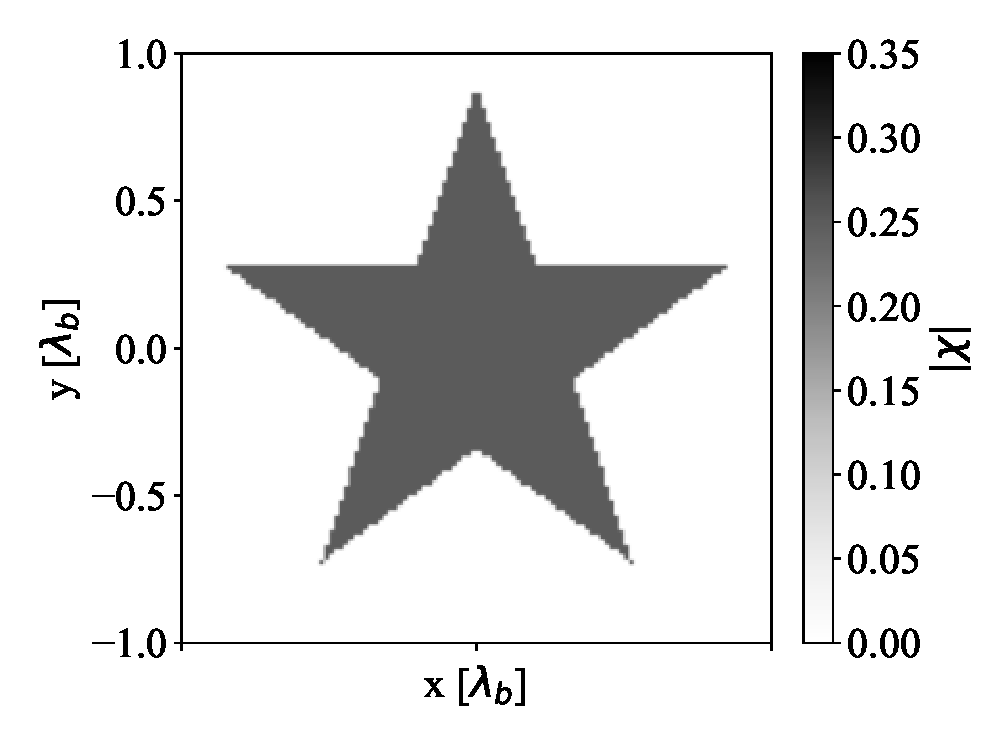
\includegraphics[width=0.33\textwidth]{./figs/shape/single/recons/0}}
                    \subfigure[LSM]{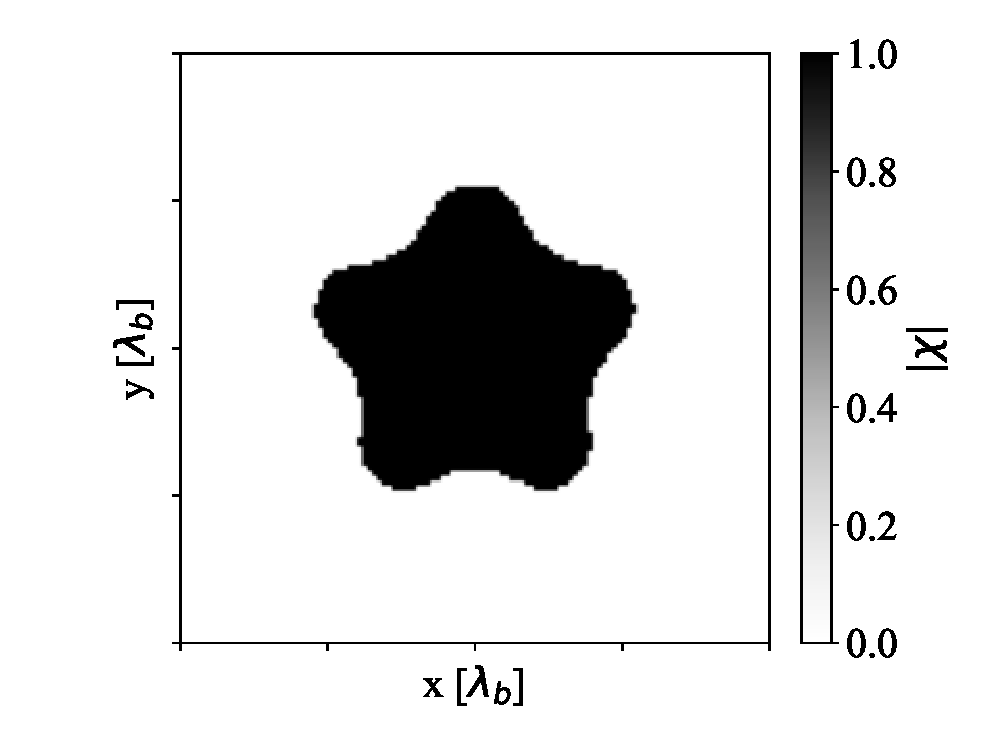
\includegraphics[width=0.33\textwidth]{./figs/shape/single/recons/1}}
                    \subfigure[OSM]{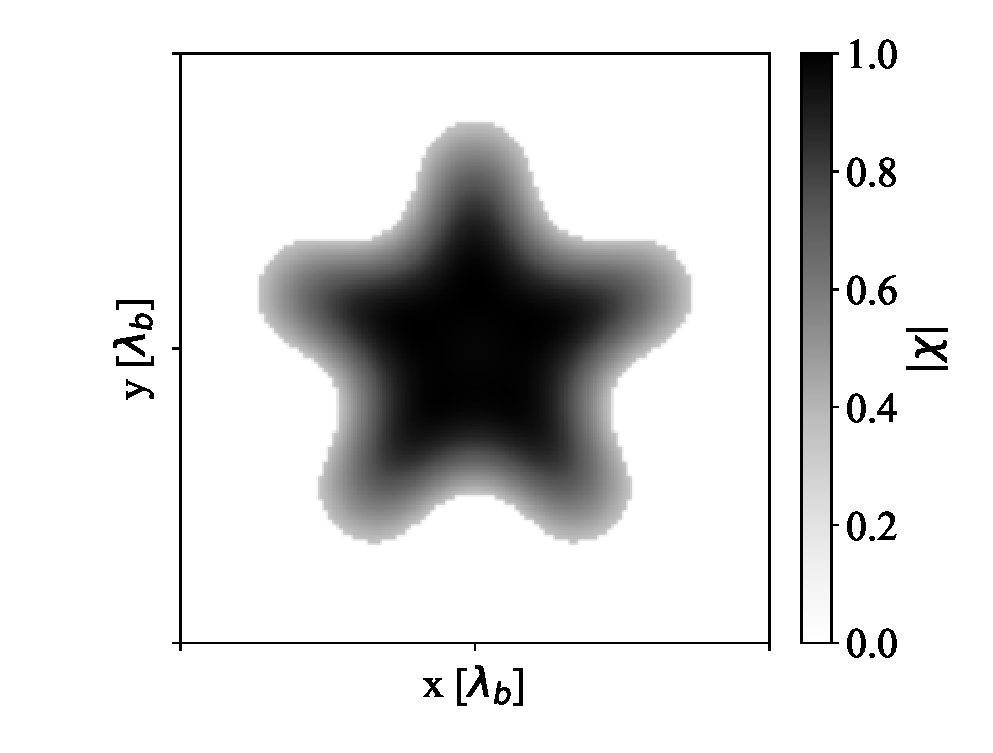
\includegraphics[width=0.33\textwidth]{./figs/shape/single/recons/2}} \\
                    \subfigure[BIM]{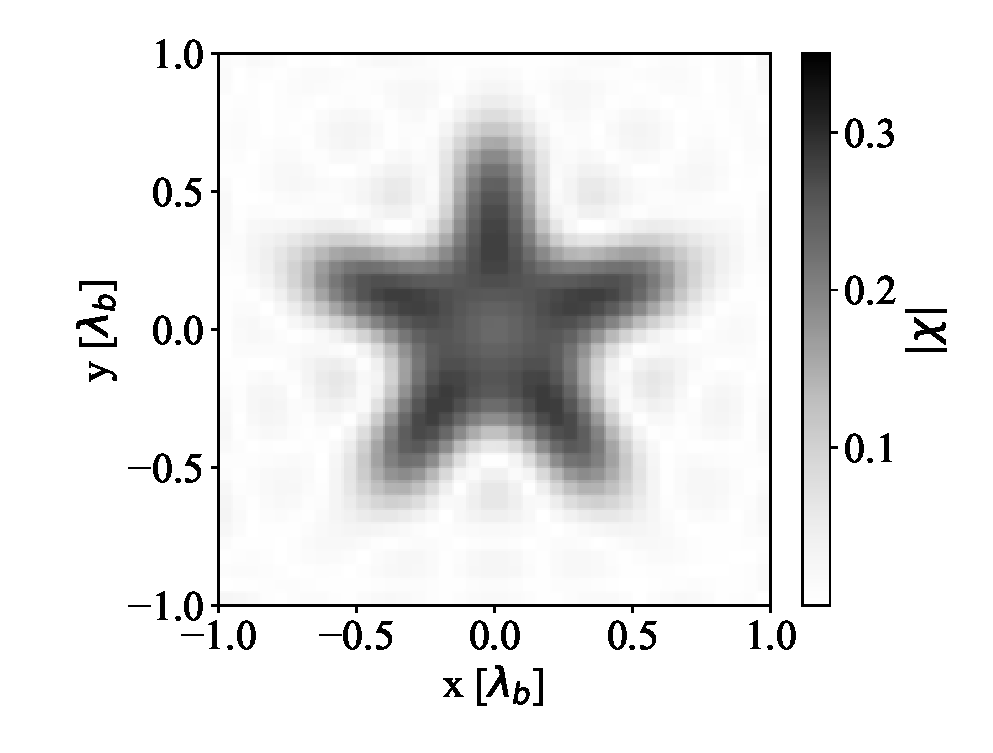
\includegraphics[width=0.33\textwidth]{./figs/shape/single/recons/3}}
                    \subfigure[CSI]{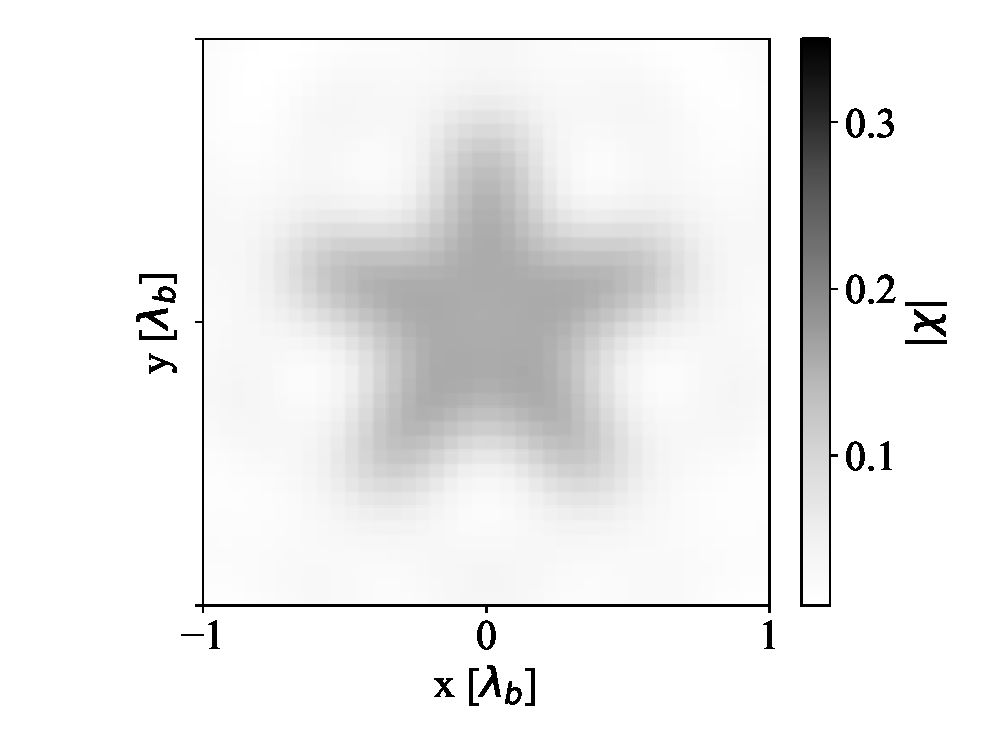
\includegraphics[width=0.33\textwidth]{./figs/shape/single/recons/4}}
                    \subfigure[SOM]{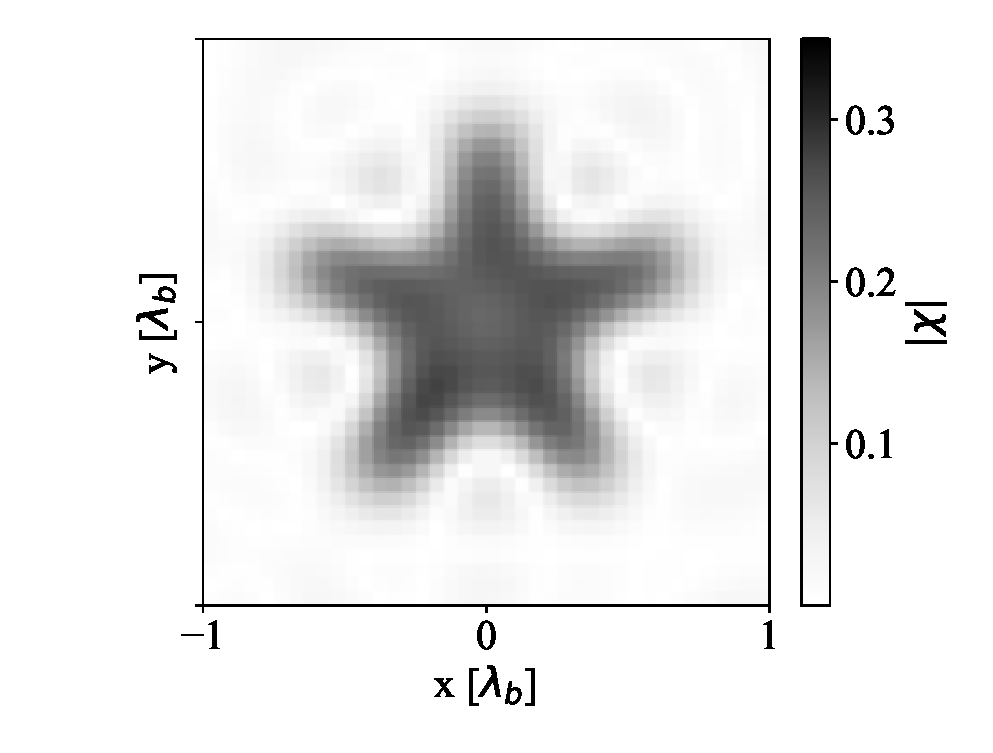
\includegraphics[width=0.33\textwidth]{./figs/shape/single/recons/5}}
                    \caption{Shape recovering study, single scatterer: ground-truth and reconstructed images by each algorithm.}
                    \label{fig:shape:single:recons}
                \end{figure*}

                % The first case study involves a single scatterer with homogeneous contrast. Fig. \ref{fig:star} illustrates the geometry of the problem. The scatterer is a five-point star with a radius of 0.1 m and a contrast of 0.5. The original image was discretized into a 100x100 pixel grid. Fig. \ref{fig:star} also shows the image reconstructed by an imaging algorithm. Table \ref{tab:star} presents the results obtained for shape and position errors. The results demonstrate that the algorithm successfully recovered the scatterer's shape with a shape error of 0.5\% and a position error of 0.1\%. These findings indicate that the algorithm accurately recovered the scatterer's shape and position.

                % \begin{figure}[!t]
                %     \centering
                %     \includegraphics[width=.8\columnwidth]{./figs/star}
                %     \caption{Single scatterer geometry.}
                %     \label{fig:star}
                % \end{figure}

                % \begin{table}[!t]
                %     \centering
                %     \caption{Results for the single scatterer case study.}
                %     \label{tab:star}
                %     \begin{tabular}{|c|c|c|}
                %         \hline
                %         Indicator & Value & Unit \\
                %         \hline
                %         $\zeta_S$ & 0.5 & \% \\
                %         $\zeta_P$ & 0.1 & \% \\
                %         \hline
                %     \end{tabular}   
                % \end{table}
			
			\subsubsection{Varying contrast}\label{sec:results:shape:varying}
			
			\subsubsection{Average performance}\label{sec:results:shape:average}
		
		\subsection{Position Detection Study}\label{sec:results:position}
		
			\subsubsection{Single scatter}\label{sec:results:position:single}
			
			\subsubsection{Multiple scatterers}\label{sec:results:position:multiple}
			
			\subsubsection{Average performance}\label{sec:results:position:benchmark}
    
    \section{Conclusion}\label{sec:conclusion}
        A conclusion section is not required. Although a conclusion may review the main points of the paper, do not replicate the abstract as the conclusion. A  conclusion might elaborate on the importance of the work or suggest applications and extensions. \cite{chen2018computational}
    
    \appendices
    
    \section*{Acknowledgment}
    
        Use the singular heading even if you have many acknowledgments. In most  cases, sponsor and financial support acknowledgments are placed in the  unnumbered footnote on the first page, not here.
    
    \bibliographystyle{IEEEtran}
    \bibliography{mybib}
    
    % \begin{IEEEbiography}[{\includegraphics[width=1in,height=1.25in,clip,keepaspectratio]{a1.png}}]
    %     {First A. Author} (M'76--SM'81--F'87) and all authors may include biographies. Biographies are often not included in conference-related papers. This author became a Member (M) of IEEE in 1976, a Senior Member (SM) in 1981, and a Fellow (F) in 1987. The first paragraph may contain a place and/or date of birth (list place, then date). Next, the author's educational background is listed. The degrees should be listed with type of degree in what field, which institution, city, state, and country, and year the degree was earned. The author's major field of study should be lower-cased. 
        
    %     The second paragraph uses the pronoun of the person (he or she) and not the author's last name. It lists military and work experience, including summer and fellowship jobs. Job titles are capitalized. The current job must have a  location; previous positions may be listed without one. Information concerning previous publications may be included. Try not to list more than three books or published articles. The format for listing publishers of a book within the biography is: title of book (publisher name, year) similar to a reference. Current and previous research interests end the paragraph. The third paragraph begins with the author's title and last name (e.g., Dr.\ Smith, Prof.\ Jones, Mr.\ Kajor, Ms.\ Hunter). List any memberships in professional societies other than the IEEE. Finally, list any awards and work for IEEE committees and publications. If a photograph is provided, it should be of good quality, and professional-looking. Following are two examples of an author's biography.
    % \end{IEEEbiography}
    
    % \begin{IEEEbiography}[{\includegraphics[width=1in,height=1.25in,clip,keepaspectratio]{a2.png}}]
    %     {Second B. Author} was born in Greenwich Village, New York, NY, USA in 1977. He received the B.S. and M.S. degrees in aerospace engineering from the University of Virginia, Charlottesville, in 2001 and the Ph.D. degree in mechanical engineering from Drexel University, Philadelphia, PA, in 2008.
        
    %     From 2001 to 2004, he was a Research Assistant with the Princeton Plasma Physics Laboratory. Since 2009, he has been an Assistant Professor with the Mechanical Engineering Department, Texas A{\&}M University, College Station. He is the author of three books, more than 150 articles, and more than 70 inventions. His research interests include high-pressure and high-density nonthermal plasma discharge processes and applications, microscale plasma discharges, discharges in liquids, spectroscopic diagnostics, plasma propulsion, and innovation plasma applications. He is an Associate Editor of the journal \emph{Earth, Moon, Planets}, and holds two patents. 
        
    %     Dr. Author was a recipient of the International Association of Geomagnetism and Aeronomy Young Scientist Award for Excellence in 2008, and the IEEE Electromagnetic Compatibility Society Best Symposium Paper Award in 2011. 
    % \end{IEEEbiography}
    
    % \begin{IEEEbiography}[{\includegraphics[width=1in,height=1.25in,clip,keepaspectratio]{a3.png}}]
    %     {Third C. Author, Jr.} (M'87) received the B.S. degree in mechanical engineering from National Chung Cheng University, Chiayi, Taiwan, in 2004 and the M.S. degree in mechanical engineering from National Tsing Hua University, Hsinchu, Taiwan, in 2006. He is currently pursuing the Ph.D. degree in mechanical engineering at Texas A{\&}M University, College Station, TX, USA.
        
    %     From 2008 to 2009, he was a Research Assistant with the Institute of Physics, Academia Sinica, Tapei, Taiwan. His research interest includes the development of surface processing and biological/medical treatment techniques using nonthermal atmospheric pressure plasmas, fundamental study of plasma sources, and fabrication of micro- or nanostructured surfaces. 
        
    %     Mr. Author's awards and honors include the Frew Fellowship (Australian Academy of Science), the I. I. Rabi Prize (APS), the European Frequency and Time Forum Award, the Carl Zeiss Research Award, the William F. Meggers Award and the Adolph Lomb Medal (OSA).
    % \end{IEEEbiography}

\end{document}

% Figure example.
\begin{figure}[!t]
    \centerline{\includegraphics[width=\columnwidth]{fig1.png}}
    \caption{Magnetization as a function of applied field. It is good practice to explain the significance of the figure in the caption.}
    \label{example}
\end{figure}

% Table example.
\begin{table}
    \caption{Units for Magnetic Properties}
    \label{table}
    \setlength{\tabcolsep}{3pt}
    \begin{tabular}{|p{25pt}|p{75pt}|p{115pt}|}
        \hline
        Symbol& Quantity& Conversion from Gaussian and \par CGS EMU to SI $^{\mathrm{a}}$ \\\hline
        $\Phi $& magnetic flux& 1 Mx $\to  10^{-8}$ Wb $= 10^{-8}$ V$\cdot $s \\
        $B$& magnetic flux density, \par magnetic induction& 1 G $\to  10^{-4}$ T $= 10^{-4}$ Wb/m$^{2}$ \\
        $H$& magnetic field strength& 1 Oe $\to  10^{3}/(4\pi )$ A/m \\
        $m$& magnetic moment& 1 erg/G $=$ 1 emu \par $\to 10^{-3}$ A$\cdot $m$^{2} = 10^{-3}$ J/T \\
        $M$& magnetization& 1 erg/(G$\cdot $cm$^{3}) =$ 1 emu/cm$^{3}$ \par $\to 10^{3}$ A/m \\
        4$\pi M$& magnetization& 1 G $\to  10^{3}/(4\pi )$ A/m \\
        $\sigma $& specific magnetization& 1 erg/(G$\cdot $g) $=$ 1 emu/g $\to $ 1 A$\cdot $m$^{2}$/kg \\
        $j$& magnetic dipole \par moment& 1 erg/G $=$ 1 emu \par $\to 4\pi \times  10^{-10}$ Wb$\cdot $m \\
        $J$& magnetic polarization& 1 erg/(G$\cdot $cm$^{3}) =$ 1 emu/cm$^{3}$ \par $\to 4\pi \times  10^{-4}$ T \\
        $\chi , \kappa $& susceptibility& 1 $\to  4\pi $ \\
        $\chi_{\rho }$& mass susceptibility& 1 cm$^{3}$/g $\to  4\pi \times  10^{-3}$ m$^{3}$/kg \\
        $\mu $& permeability& 1 $\to  4\pi \times  10^{-7}$ H/m \par $= 4\pi \times  10^{-7}$ Wb/(A$\cdot $m) \\
        $\mu_{r}$& relative permeability& $\mu \to \mu_{r}$ \\
        $w, W$& energy density& 1 erg/cm$^{3} \to  10^{-1}$ J/m$^{3}$ \\
        $N, D$& demagnetizing factor& 1 $\to  1/(4\pi )$ \\\hline
        \multicolumn{3}{p{251pt}}{Vertical lines are optional in tables. Statements that serve as captions for the entire table do not need footnote letters. }\\
        \multicolumn{3}{p{251pt}}{$^{\mathrm{a}}$Gaussian units are the same as cg emu for magnetostatics; Mx $=$ maxwell, G $=$ gauss, Oe $=$ oersted; Wb $=$ weber, V $=$ volt, s $=$ second, T $=$ tesla, m $=$ meter, A $=$ ampere, J $=$ joule, kg $=$ kilogram, H $=$ henry.}
    \end{tabular}
    \label{tab1}
\end{table}

